\documentclass[a4paper]{article}
\usepackage[affil-it]{authblk}
\usepackage[backend=bibtex,style=numeric]{biblatex}
\usepackage{ctex}
\usepackage{geometry}
\usepackage{graphicx}
\usepackage{float}
\geometry{margin=1.5cm, vmargin={0pt,1cm}}
\setlength{\topmargin}{-1cm}
\setlength{\paperheight}{29.7cm}
\setlength{\textheight}{25.3cm}

\addbibresource{citation.bib}

\begin{document}
% =================================================
\title{Proj: report}

\author{陈昊鹏  3220103347@zju.edu.cn}
\affil{数学与应用数学(强基计划)}


\date{Due time: \today}

\maketitle
% ============================================
\subsection*{A.}
$N=6,11,21,41,81$,对于每一个N对应的三阶PP曲线拟合,区间中点误差最大值依次如图中所示:
\begin{figure}[H]
    \centering
    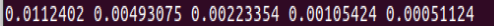
\includegraphics[width=0.7\textwidth]{A.png}
    \caption{the max-norm of the interpolation error at mid-points of subintervals for each N}
    \label{Fig}
\end{figure}
对于每一个N,插值函数图像如下:
\begin{figure}[H]
    \centering
    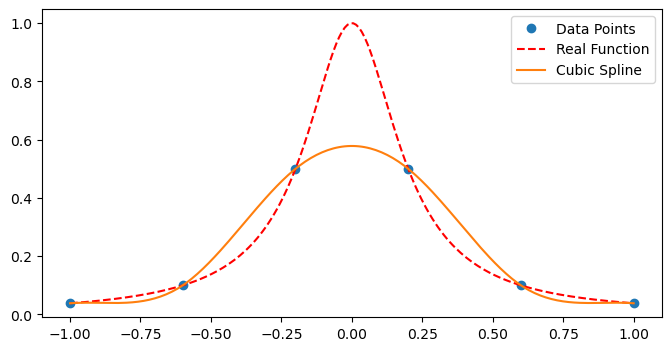
\includegraphics[width=0.7\textwidth]{N=6.png}
    \caption{interpolation spline with N=6}
    \label{Fig}
\end{figure}
\begin{figure}[H]
    \centering
    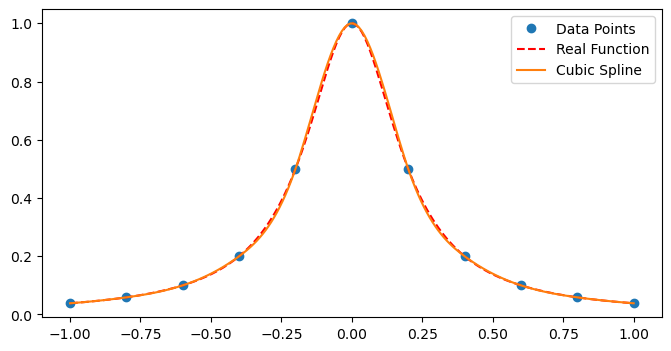
\includegraphics[width=0.7\textwidth]{N=11.png}
    \caption{interpolation spline with N=11}
    \label{Fig}
\end{figure}
\begin{figure}[H]
    \centering
    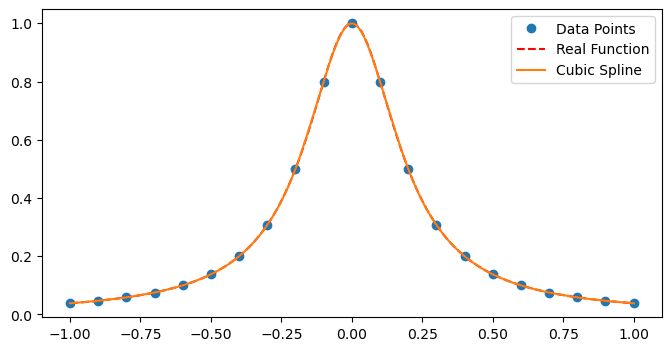
\includegraphics[width=0.7\textwidth]{N=21.png}
    \caption{interpolation spline with N=11}
    \label{Fig}
\end{figure}
\begin{figure}[H]
    \centering
    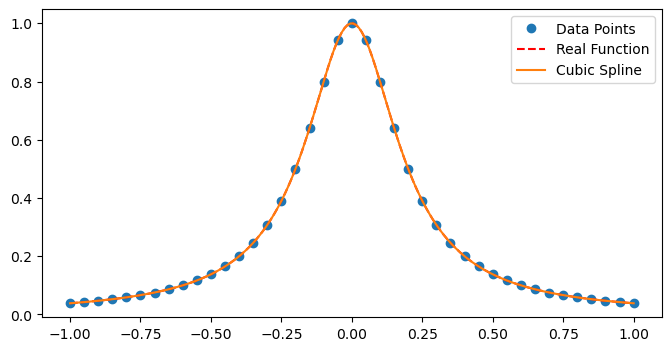
\includegraphics[width=0.7\textwidth]{N=41.png}
    \caption{interpolation spline with N=41}
    \label{Fig}
\end{figure}
\begin{figure}[H]
    \centering
    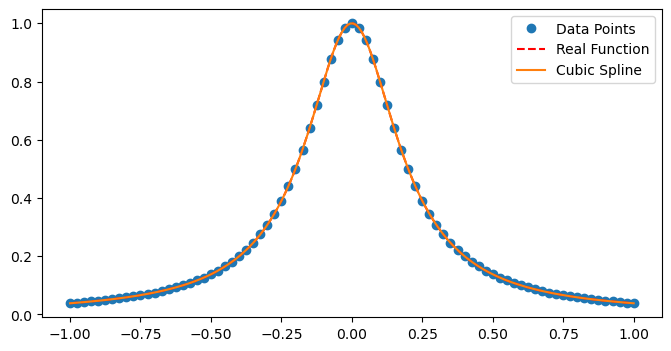
\includegraphics[width=0.7\textwidth]{N=81.png}
    \caption{interpolation spline with N=81}
    \label{Fig}
\end{figure}
综上可看出龙格现象被极大避免了.

\subsection*{C.}
用二阶B样条在$i-\frac{11}{2},i=1,...,10$插值的函数图像为:
\begin{figure}[H]
    \centering
    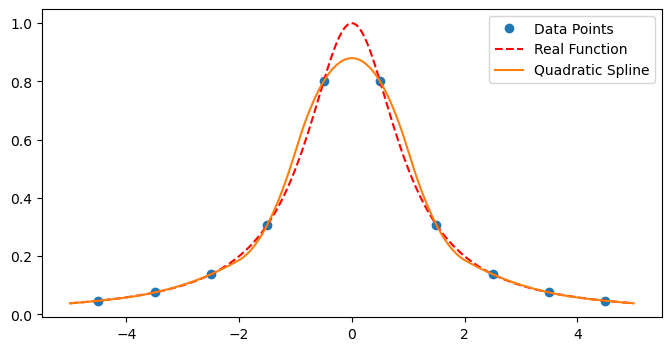
\includegraphics[width=0.7\textwidth]{C_QuadraticSpline.png}
    \caption{Quadratic Spline}
    \label{Fig}
\end{figure}
用三阶B样条在$i-6,i=1,...,11$插值的函数图像为:
\begin{figure}[H]
    \centering
    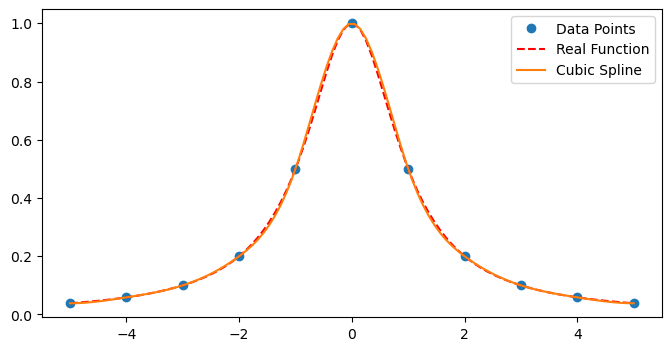
\includegraphics[width=0.7\textwidth]{C_CubicSpline.png}
    \caption{Cubic Spline}
    \label{Fig}
\end{figure}

\subsection*{D.}
用三阶B样条拟合后的曲线在给定点处的误差值:
\begin{figure}[H]
    \centering
    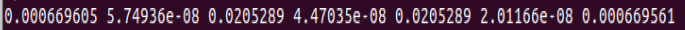
\includegraphics[width=0.7\textwidth]{D_Cubic.png}
    \caption{the interpolation error of Cubic Spline at given sites}
    \label{Fig}
\end{figure}
用二阶B样条拟合后的曲线在给定点处的误差值:
\begin{figure}[H]
    \centering
    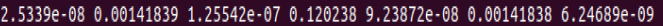
\includegraphics[width=0.7\textwidth]{D_Quadratic.png}
    \caption{the interpolation error of Quadratic Spline at given sites}
    \label{Fig}
\end{figure}
可以看到,用三阶B样条拟合后的曲线在$-3,0,3$处的误差较小,用二阶B样条拟合后的曲线在
$-3.5,-0.5,0.5,3.5$处的误差较小.这是因为用三阶B样条曲线拟合时,插值点选在$-3,0,3$,
用二阶B样条曲线拟合时插值点选在$-3.5,-0.5,0.5,3.5$.总体来看用三阶B样条拟合后的曲线
误差更小.

\subsection*{E.}
对心形曲线,等距节点拟合和使用累计曲线长度进行拟合的效果如下:
\begin{figure}[H]
    \centering
    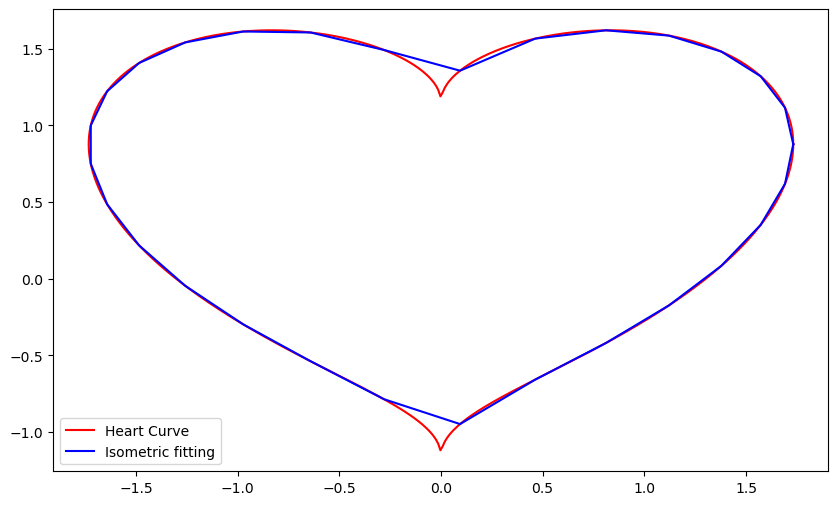
\includegraphics[width=0.7\textwidth]{E1_IsometricFitting.png}
    \caption{heart curve Isometric Fitting}
    \label{Fig}
\end{figure}
\begin{figure}[H]
    \centering
    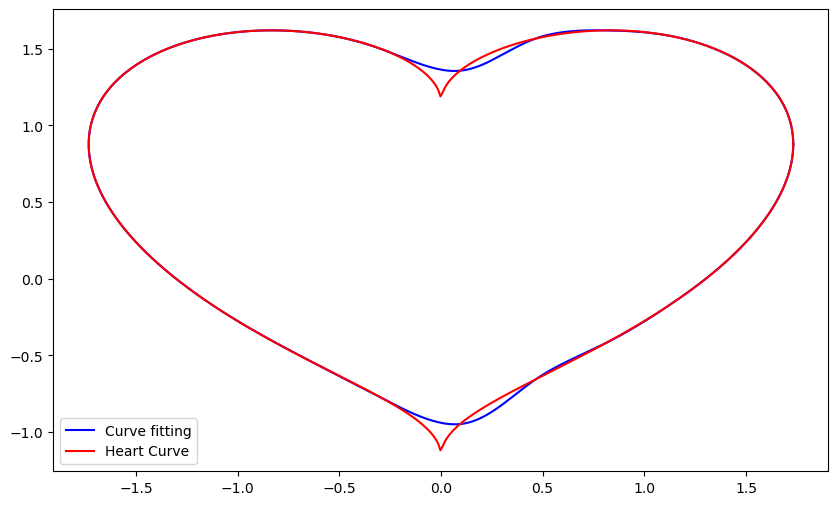
\includegraphics[width=0.7\textwidth]{E1_CurveFitting.png}
    \caption{heart curve Curve Fitting}
    \label{Fig}
\end{figure}
对第二种曲线,等距节点拟合和使用累计曲线长度进行拟合的效果如下:
\begin{figure}[H]
    \centering
    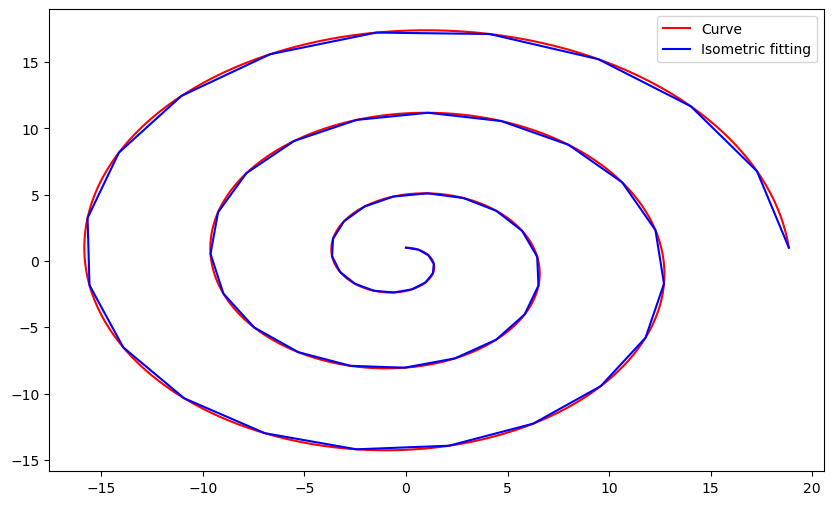
\includegraphics[width=0.7\textwidth]{E2_IsometricFitting.png}
    \caption{second curve Isometric Fitting}
    \label{Fig}
\end{figure}
\begin{figure}[H]
    \centering
    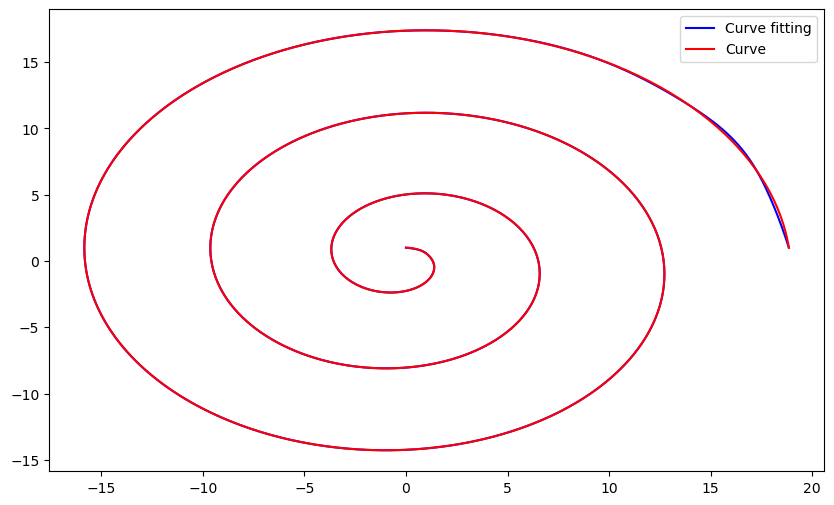
\includegraphics[width=0.7\textwidth]{E2_CurveFitting.png}
    \caption{second curve Curve Fitting}
    \label{Fig}
\end{figure}
对第三种曲线,等距节点拟合和使用累计曲线长度进行拟合的效果如下:
\begin{figure}[H]
    \centering
    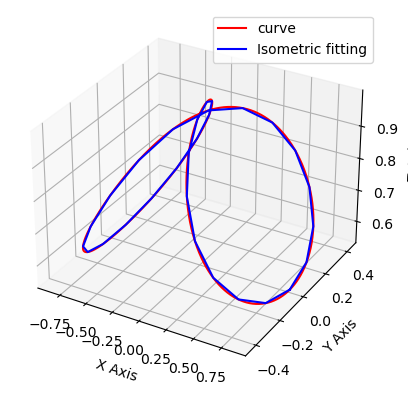
\includegraphics[width=0.7\textwidth]{E3_IsometricFitting.png}
    \caption{third curve Isometric Fitting}
    \label{Fig}
\end{figure}
\begin{figure}[H]
    \centering
    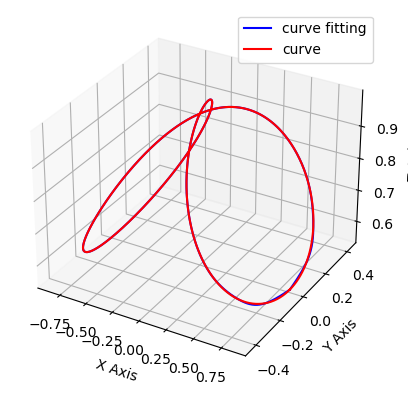
\includegraphics[width=0.7\textwidth]{E3_CurveFitting.png}
    \caption{third curve Curve Fitting}
    \label{Fig}
\end{figure}

\subsection*{F.}
$n=1$时,table of divided difference of truncated power functions如下图所示:
\begin{figure}[H]
    \centering
    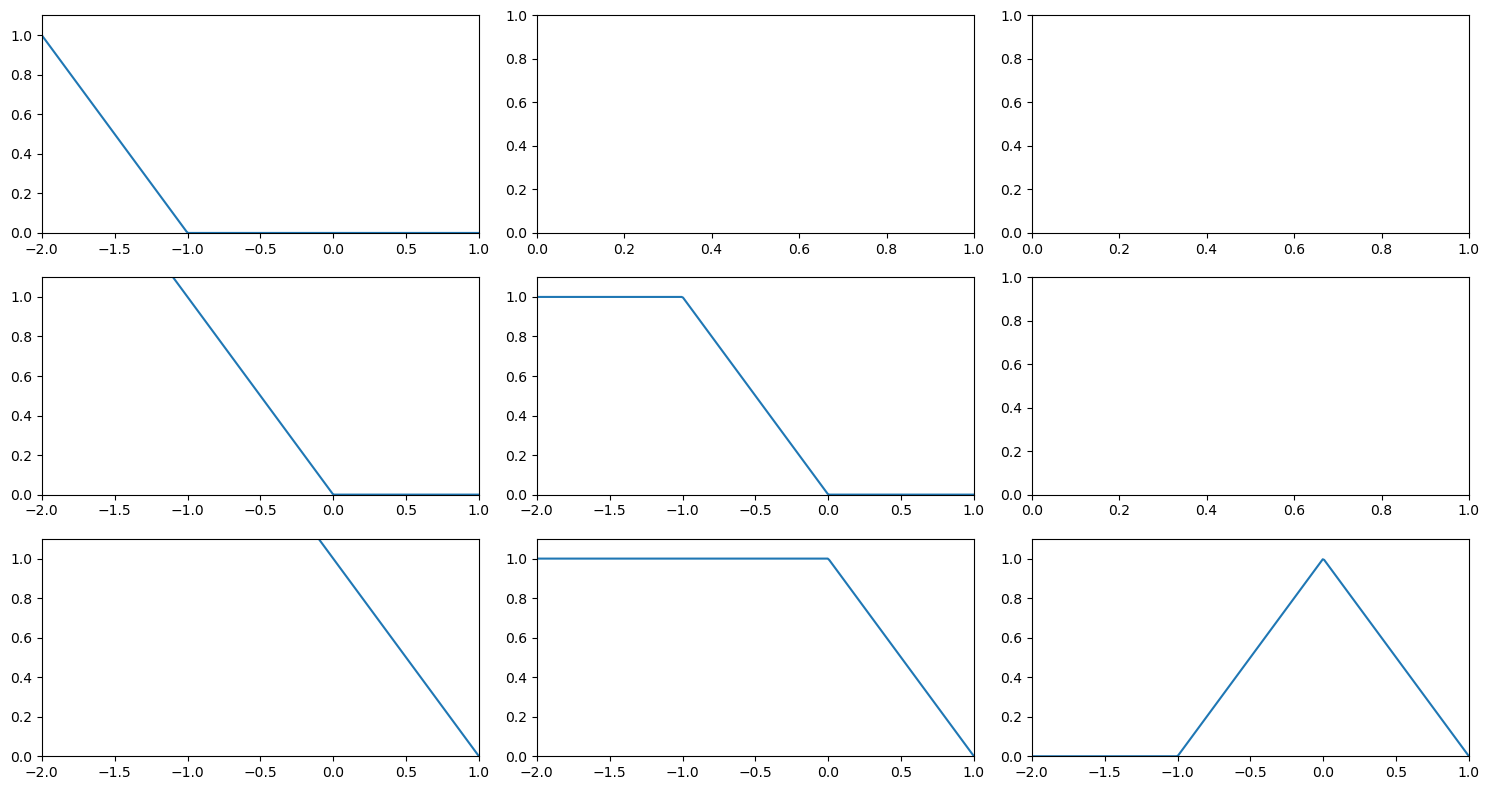
\includegraphics[width=0.7\textwidth]{F1.png}
    \caption{table of divided difference when $n=1$}
    \label{Fig}
\end{figure}
$n=2$时,table of divided difference of truncated power functions如下图所示:
\begin{figure}[H]
    \centering
    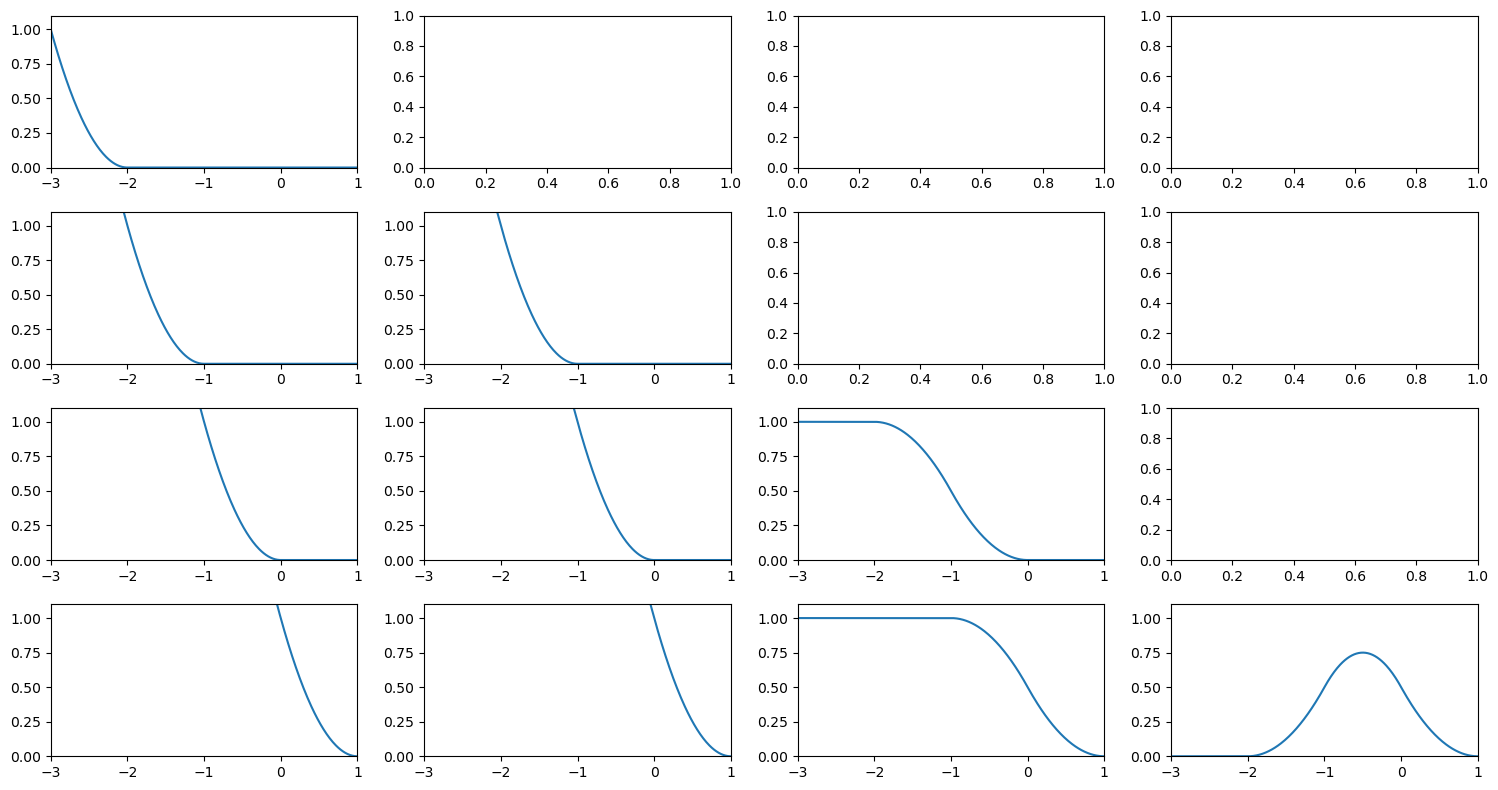
\includegraphics[width=0.7\textwidth]{F2.png}
    \caption{table of divided difference when $n=2$}
    \label{Fig}
\end{figure}

\end{document}